\subsection{Approach}

dsfasdfasdfasdfasdf
roll assignment with algorithms 


\subsection{Role Assignment}

As stated, the purpose of this research is to prove that subtask division can
be accomplished based on knowledge of robot capabilities. To prove this, we are
developing an exploration system in which robots with different hardware and
capabilities will work together to accurately explore and map a complex region
of space. Through the definition of individual attributes and the sharing of
those attributes, each robot will search and map regions of space that it is
capable of maneuvering. Instead of simple binary mapping of the region, 1 =
free space and 0 = obstacle, each robot will mark the region that it has
explored and can maneuver through this a specific identifier. This gives the
region itself a bit of information as well as allows other robots to help
determine if they are capable of maneuvering as well.
Once a robot comes to an obstacle or region that it cannot maneuver around,
it will evaluate which team members are capable of doing so and mark that space
for the capable robots to explore. Due to time limitations on this project,
instead of relying on complex perceptive capabilities to evaluate which robots
could explore that region, the utilization of QR codes on unique obstacles will
illustrate attribute sets necessary for that exploration.

\begin{figure}
    \centering
    \begin{subfigure}[b]{0.15\textwidth}
        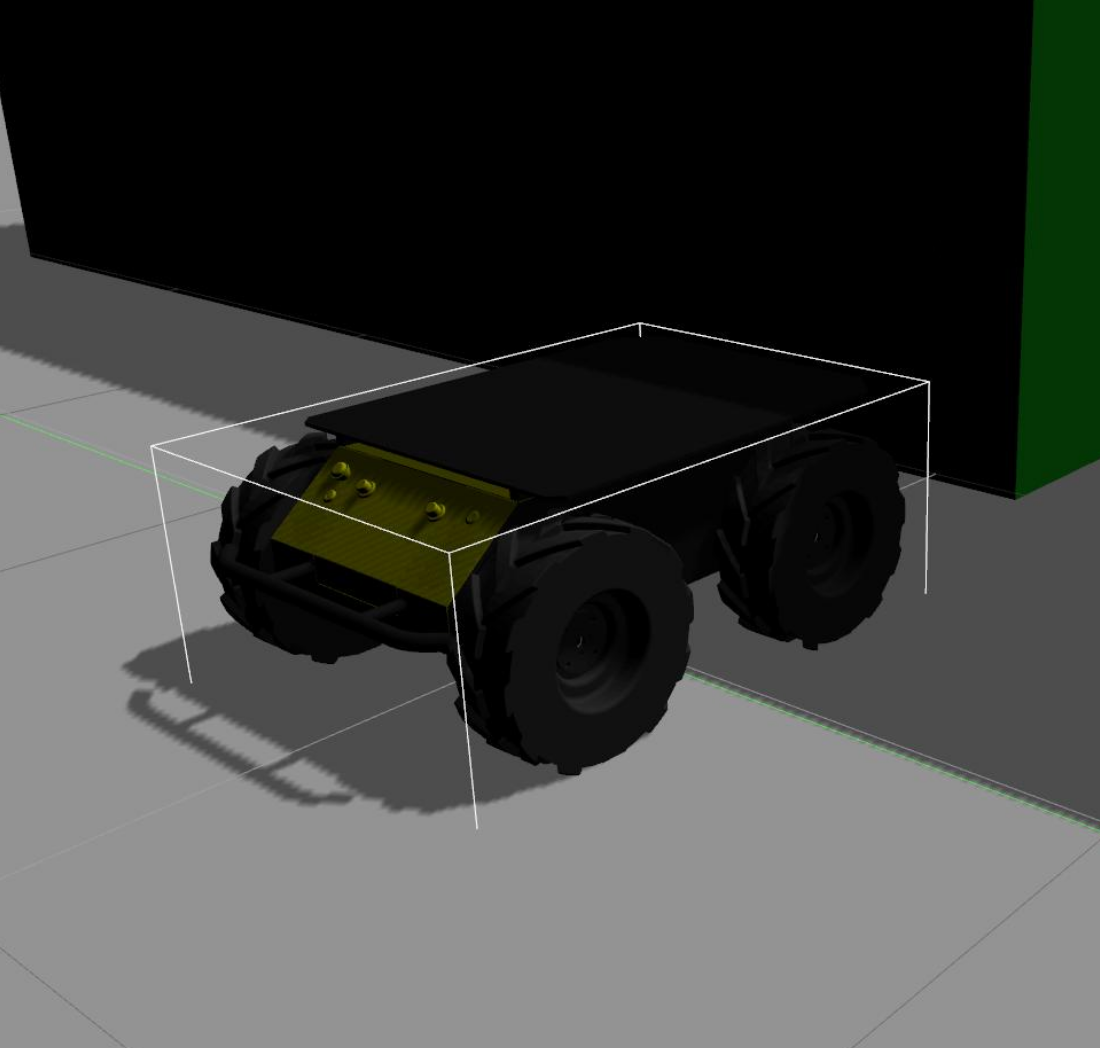
\includegraphics[width=\textwidth]{bot1}
        \caption{Husky bot}
        \label{fig:bot1}
    \end{subfigure}
    \begin{subfigure}[b]{0.15\textwidth}
        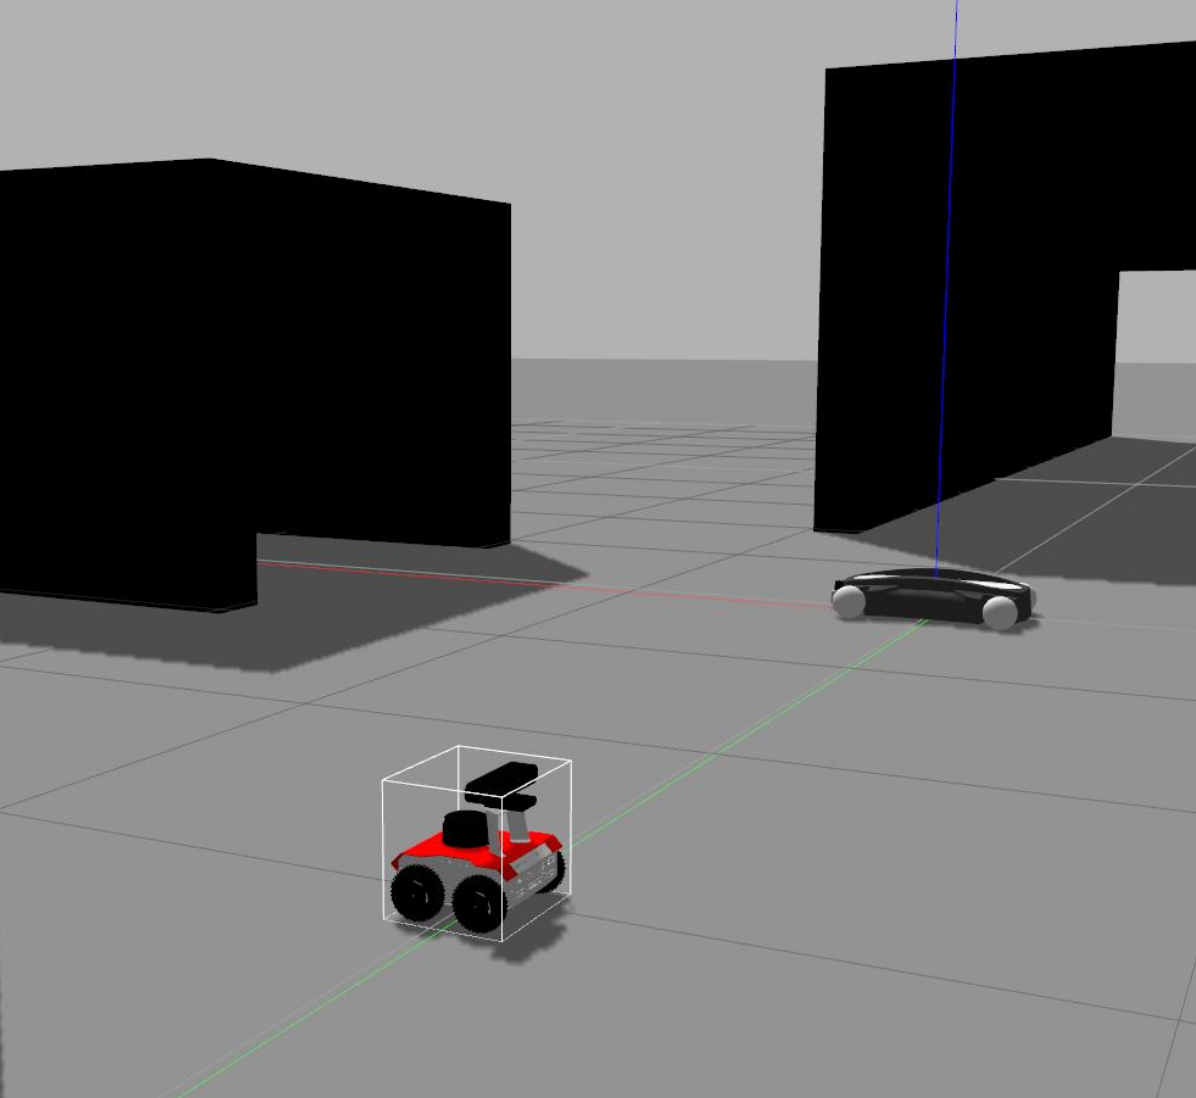
\includegraphics[width=\textwidth]{bot2}
        \caption{Rosbot}
        \label{fig:bot2}
    \end{subfigure}
    \begin{subfigure}[b]{0.15\textwidth}
        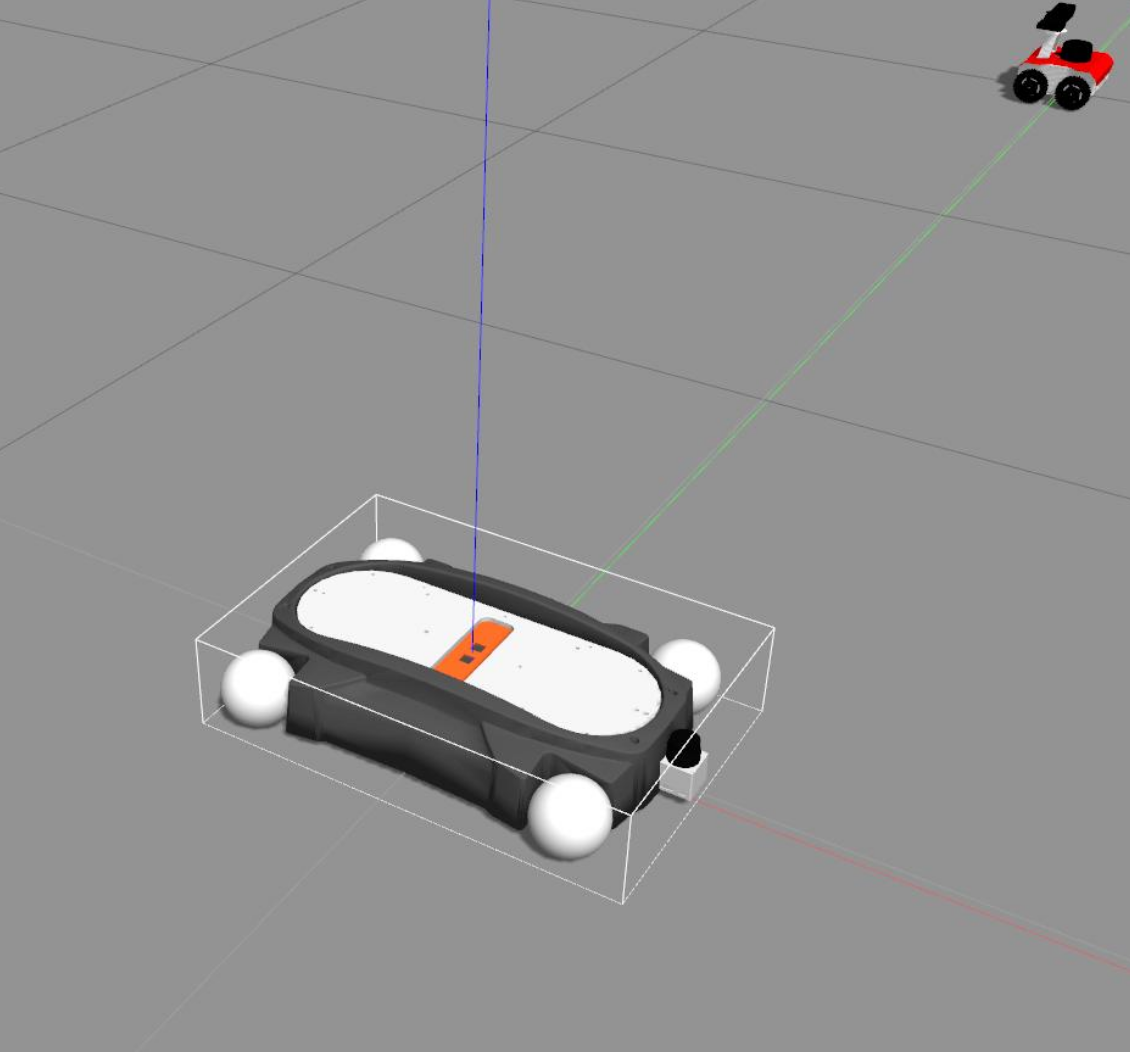
\includegraphics[width=\textwidth]{bot3}
        \caption{Youbot}
        \label{fig:bot3}
    \end{subfigure}
    \caption{Three commonly used robots with very different shapes and sizes.}\label{fig:bots}
\end{figure}

As an individual working in a cooperative operation, knowing the capabilities
of you and your teammates is necessary to the division of tasks. This idea
provides the basis for this proposed research. As homogeneous multi-robot systems
are inherently limited based on the capabilities of the specific robot,
it makes sense to venture down a heterogeneous avenue. A lot of research
has gone into heterogeneous multi-robot systems in the past few years, but a
common trend amongst most of them is that the model is built for the specific
platforms that are to be used. This proposed research is meant to provide the
groundwork for a heterogeneous model that allows for the insertion of a
robots with different skill sets with the purpose of enhancing the overall
capability of the system. This framework would allow for a variety of models
to be built on top of it, with a variety of hardware. Researchers wanting to
build a specific system could allocate funds and resources to build each member
to accomplish a portion of the overall task, possibly allowing for more cost
efficiency and remove unnecessary redundancy. The main challenge in this
research will be finding the optimal way to reassign tasks based on defined
capabilities of each robot in the system. This brings up a secondary, more basic,
challenge of defining robot’s characteristics in a simple yet comprehensive manor.
All-in-all, this research acts as a proof of concept for task division based on member
attributes, or individual robots capabilities, and will allow for a high degree of
heterogeneous utilization and multi-robot model expansion.

\begin{figure}[H]
  \centering
    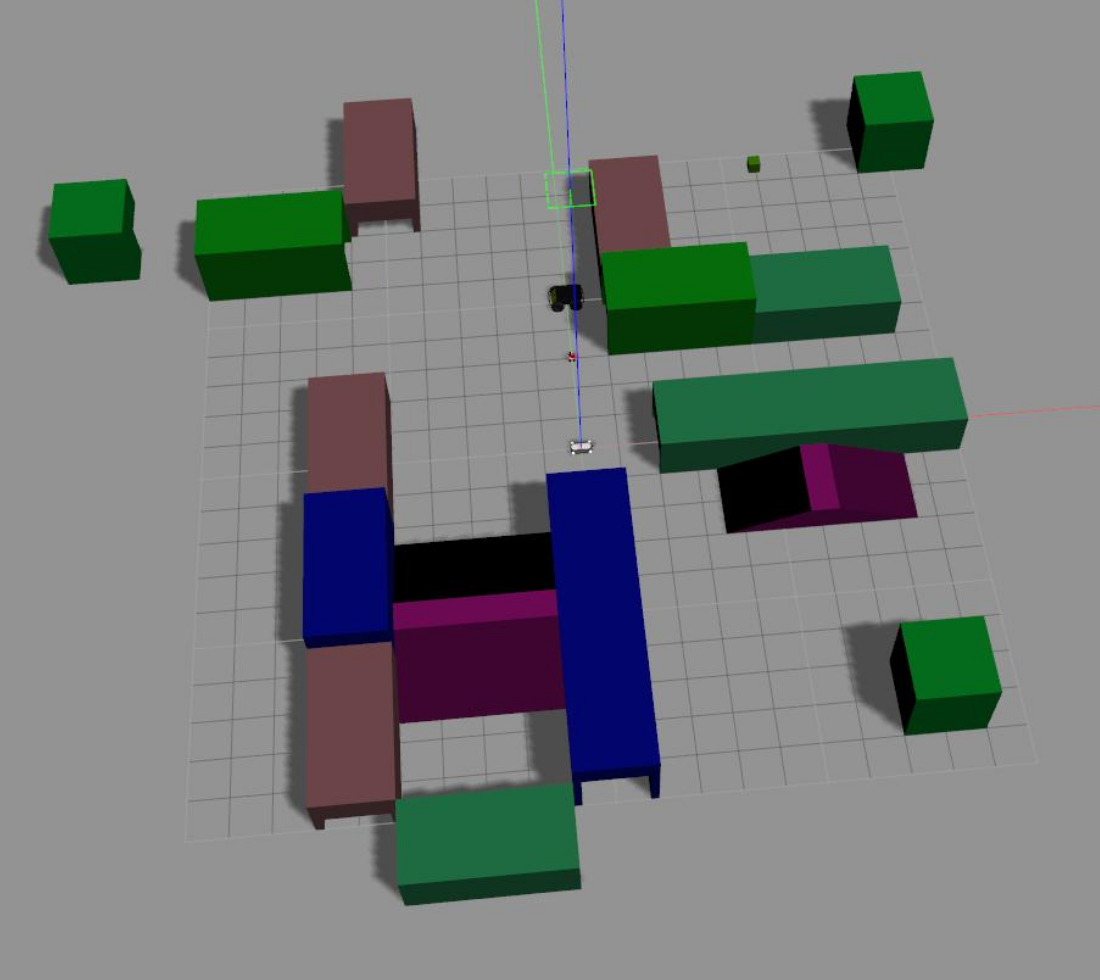
\includegraphics[width=0.5\textwidth]{map2}
  \caption{This is a caption of this figure.}
  \label{fig:something1}
\end{figure}

\begin{figure}[H]
  \centering
    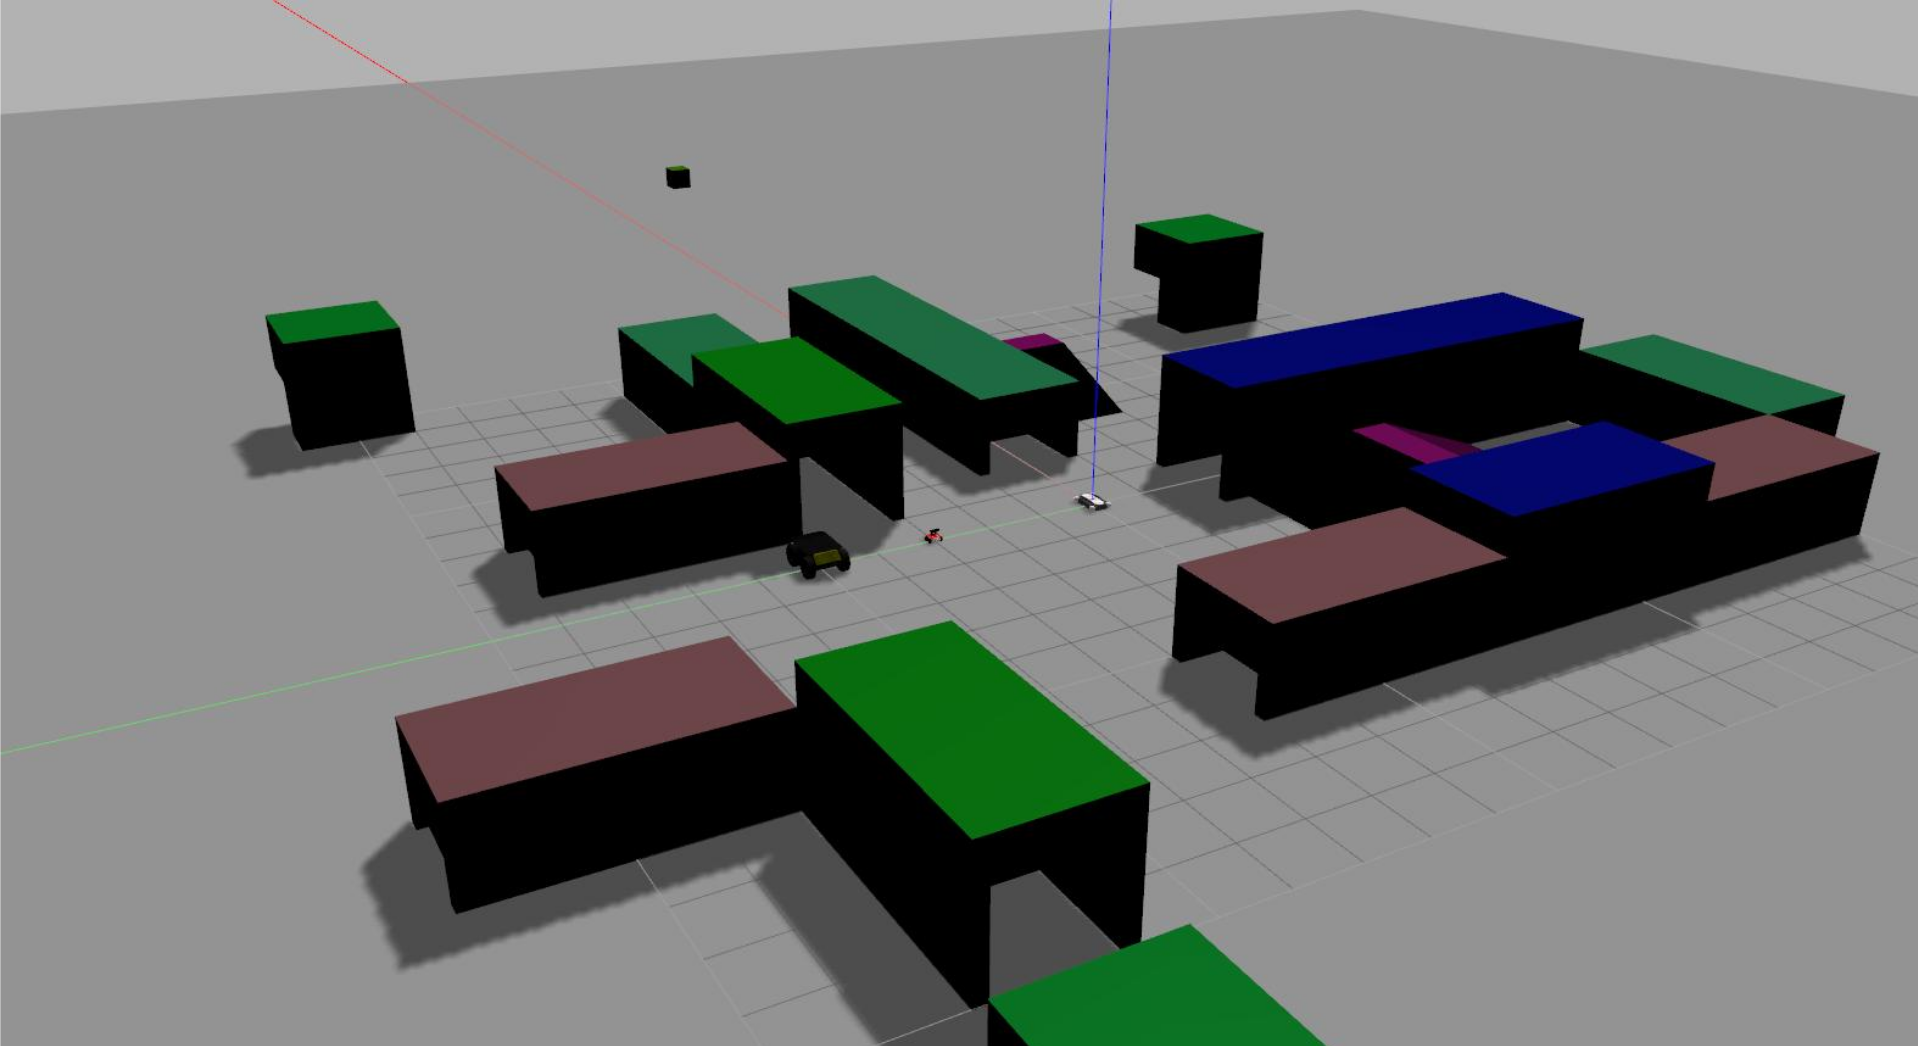
\includegraphics[width=0.5\textwidth]{map1}
  \caption{This is a caption of this figure.}
  \label{fig:something2}
\end{figure}

\subsection{Algorithms}

The exploration model is a heuristic based algorithm that encourages the robot to explore
away from its neighbors to ensure maximum coverage and remove possibility of initial
redundant searches.

- DFS
- A*

Lorem ipsum dolor sit amet, consectetur adipiscing elit,
sed do eiusmod tempor incididunt ut labore et dolore magna aliqua. Ut enim ad
minim veniam, quis nostrud exercitation ullamco laboris nisi ut aliquip ex ea
commodo consequat. Duis aute irure dolor in reprehenderit in voluptate velit
esse cillum dolore eu fugiat nulla pariatur. Excepteur sint occaecat cupidatat
non proident, sunt in culpa qui officia deserunt mollit anim id est laborum.

% this section has 3 figures together

\subsection{Testing Framework}

After exploring a set of options to test this idea, the best place to go was to the drawing
board. Taking a step back it was decided that pushing to get straight into hardware testing
was a poor decision and the underlying concept of heterogeneous task reallocation based on
capabilities needed to be tested at the lowest of levels. To do this, the creation of a testing
framework in roscpp was necessary. This framework allows for easy addition of robots by simply
adding the details for the new robot in the xml robots launch file. To add any additional information
yaml files can be used to set rosparams, just as was done here for robot capabilties. By configuring
the launch file with the proper robots, one can edit the one robot launch file to have each robot launch
any set of nodes that would exist in each robot's namespace. This allows for testing of a completely
decentralized algorithm in a centralized system. The reason this was done was because of the difficulty
of getting a multimaster architecture working within gazebo.
